\section{Component Densities}


\begin{figure}[h!]
\begin{center}
	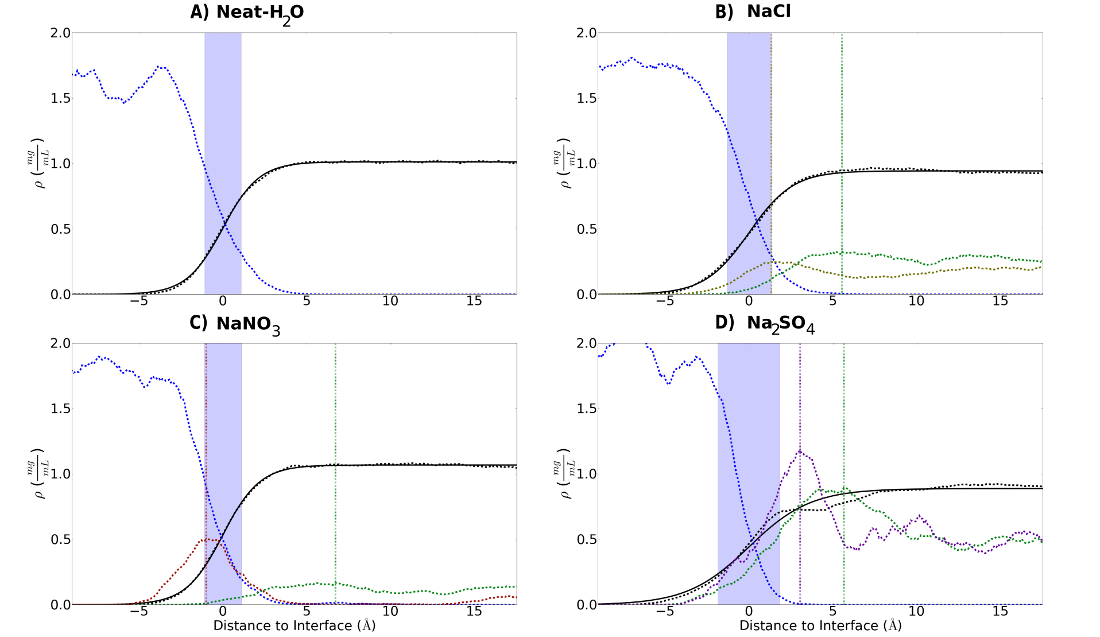
\includegraphics[scale=0.16]{images/densities.png}
	\caption{Aqueous salt and CCl$_4$ density profiles. The gibbs dividing surface location, $z_0$, were designated as the 0.0 $\AA$ location, and all lineshapes are plotted as distances to the gibbs interface. Neat-H$_2$O (A), NaCl (B), NaNO$_3$ (C), and Na$_2$SO$_4$ (D) salt-system densities are plotted with the water-oxygen density (dashed black) and the corresponding fitted lineshape (solid black). Each interfacial width, $d$, is designated as a highlighted blue region of width $d$ centered about $z_0$. The CCl$_4$ (dashed blue), Na$^+$ cation (dashed green) and respective anion densities are also shown for each system. The scaling of the cation (10x) and anion (5x) densities was used to clarify their peak and trough locations. The maxima of the ionic components are marked with dashed vertical lines of the same colors to show relative component locations within the interfacial region.}
	\label{fig:density-plots}
\end{center}
\end{figure}

The component density profiles of each system were calculated to study the effects of adding salts and to find deviations from the neat-H$_2$O/CCl$_4$ system. The water density profile of each system was fitted to a hyperbolic tangent (Eq. \ref{tanh_fit}), and the all the density profiles were plotted as distances from each of the gibbs dividing surface locations, $z_0$. The resulting plots are shown in figure \ref{fig:density-plots} with letter labels that will be used to refer to the systems. $z_0$ of each system was shifted to a location of 0.0 $\AA$, and the interfacial thickness, $d$, is visualized by a blue shaded region of the respective thickness centered about $z_0$. The widths of the interfacial regions for the neat-H$_2$O (A), NaCl (B), NaNO$_3$ (C), and Na$_2$SO$_4$ (D) systems are 2.16, 2.62, 2.20, and 3.69 $\AA$ respectively. In each of the salt solutions, the peak in the anionic density profile occurs closer to the CCl$_4$ phase than the corresponding cationic peak. Various parameters of interest such as the interfacial thicknesses, ionic component locations, and relative distances between the peaks of the ion profiles are collected in table \ref{system-params}.

\begin{table}[htdp]
	\begin{center}
	\begin{tabular}{|c||c|c|c|c|}
		\hline
		System & $d$ & Anion & Cation & Anion-Cation Distance \\ \hline
		Neat-H$_2$O & 2.16 & - & - & - \\ 
		NaCl & 2.62 & 1.33 & 5.53 & 4.20 \\
		NaNO$_3$ & 2.20 & -0.99 & 6.71 & 7.70 \\
		Na$_2$SO$_4$ & 3.69 & 3.04 & 5.64 & 2.60 \\
		\hline
	\end{tabular}
	\end{center}
	\caption{Aqueous salt system density parameters. Interfacial widths, $d$, and the locations of the maxima of the density profiles for each ionic component are listed for the simulated salt systems. The relative distances between the anion and cation density peak locations are listed to show how the different anions affect the relative location of their cationic counterions.}
	\label{system-params}
\end{table}

The oscillations in the surface density profiles of water and the adjoining organic liquid phase have been noted previously and attributed to thermal capillary waves on a larger length-scale than the simulated system size.\cite{Chang1996} The same work also made note that the interfacial thickness is size-dependent on the interfacial surface area. Increasing the surface area dimensions should cause an increase in the interfacial width. Two works on the water-CCl$_4$ surface offer direct comparison of this.\cite{Chang1996,Hore2008} In comparing the interfacial widths, there is an increase in width as the system cross-sectional area is increased. This phenomenon implies that care must be taken when making quantitative comparisons between simulation studies.

System A is the acting benchmark and has been simulated previously by various groups. Deviations in width of the interface from the pure-water system can be attributed to the added ions in the solution. In comparing the three salt solutions, any differences in those systems are anionic in nature because the cation of each system was kept the same. System B is the simplest of the three salts with a monatomic and monovalent anion. The peak of the anion density profile is within the aqueous phase and is found on the aqueous-side of the interfacial width, $d$. The location of the cation density peak is, as mentioned above, deeper into the aqueous phase than the anion by over 4 $\AA$. This layering of ions within the aqueous phase is attributed to the break in the anisotropy of the field of the bulk region upon introduction of the second (organic) phase. The more polarizable and negatively charged anions move towards the interface to effectively screen the charge of the second phase and the more highly ordered water structure. The counterions then are drawn towards the negative charge built up by the anions to create the second ion density peak. The overall shape of the water profile in system B is relatively unaffected as the bulk water density is unchanged, and the width of the interface is increased by 18\% from that of system A. 

System C introduces the monovalent, polyatomic nitrate anion. The location preference of nitrate is a contentious subject that has been studied much in recent years. Experimental works have been performed using a few surface-sensitive techniques. One work used sum frequency generation (SFG), which detected structural changes in the hydrogen-bonding network in the presence of the anion that affect the SFG signal intensity from the interface, but could not create the anion density profile\cite{Schnitzer2000}. The same work found SFG intensity enhancement for hydrogen-bonded water following a trend of H$_2$SO$_4\ge$ HCl $>$ HNO$_3$. Strengthening of the interfacial hydrogen-bonding structure of water would allow it to further penetrate into a second phase, thus widening the interface region, and enhancing the SFG intensity from the interface for hydrogen-bonded species. We find the same trend when comparing interfacial widths from our simulations. In the case of the nitrate anion location, however, the SFG studies stopped short of reporting a concentration profile. A recent X-ray photoemission spectroscopy study was performed to specifically determine the nitrate concentration profile for the water-vapor interface, and reported the current differences of opinion between recent experiment and simulation.\cite{Brown2009} The XPS results reported a surface depletion of the nitrate anion relative to the bulk, similar to previous MD simulations of the same systems. Other works find similar nitrate surface depletions,\cite{Otten2007} but were performed on the liquid-vapor interface, and help to contrast the effect of the presence of an organic phase as in the present work. We find a surface enhancement of the nitrate anion located far to the organic side of the interface. The nitrate density peak is located the furthest out from the aqueous phase of the three salt systems. The location of the sodium cation peak is a significant distance further into the bulk from the anion than either of systems B and D. Such surface location and enhancement of the nitrate ion suggests a very strong interaction with the interface waters, breaking the hydrogen-bonding network near to the organic phase, and also strongly screening the field of the CCl$_4$ molecules from the interface. This accounts for the narrower interfacial width as the water can no longer extend a bonded network into the organic phase. However, as the water is strongly interacting with the nitrate and effectively screening the surface charge from the bulk, the cation is less attracted to the interface and the ionic double-layer is widened. Xu, et al, studied this phenomena finding a lack of ion-pairing of various nitrates at the air-water interface.\cite{Xu2009} They found that solvation from an abundance of water at the interface weakens coulombic forces between ions, leading to greater cation-anion separation. They concluded that the surface nitrate is dehydrated, and the water provides adequate shielding of the ionic coulombic interactions. It is reasonable to assume that this same effect may cause the greater cation-anion separation at the interface of system C, even in the presence of the organic phase.

The widest interface is that of the NaSO$_4$ solution in system D, indicating that the SO$_4^{2-}$ ions act to affect the hydrogen bonding network between the surface waters. The location of the sulfate density enhancement is the furthest into the aqueous bulk of the three anions, and the divalent and highly polarizable nature of the anion appears to attract the counterion closest for the narrowest sub-surface ionic double-layer. This attraction is likely coulombic, and the charge screening that separates the ion pairs in system C is not present in system D. Although the geratest concentration enhancement is further into the bulk region, seemingly outside the region designated by the width, the water network is still greatly enhanced. This has been verified by an increase in SFG response of the surface waters relative to the neat-water system in a recent work by this group\cite{McFearin2009}


%Ionic density profiles were fitted by adding a gaussian function to the hyperbolic tangent function (Eq. \ref{ion_fit}) to more closely capture the concentration enhancement excess near or within the interfacial region. The lineshape parameters for each salt system are shown in table \ref{ion_params}.

%\begin{table}[htdp]
	%\begin{center}
	%%system; Anion: (a,b,c,Z0,d); Cation: (a,b,c,Z0,d)
	%\begin{tabular}{c|c|c|c|c|c|c|c|c|c|c|}
		%\cline{2-11}
		%\multicolumn{1}{c|}{} & \multicolumn{5}{c}{Anion} & \multicolumn{5}{|c|}{Cation} \\ 
		%\cline{1-11}
		%\multicolumn{1}{|c|}{System} & $a$ & $b$ & $c$ & $z_0$ & $d$ & $a$ & $b$ & $c$ & $z_0$ & $d$ \\ \hline
		%\multicolumn{1}{|c|}{NaCl} & 0.464 & -1.726 & 1.361 & -3.190 & 1.928 & -0.257 & -8.252 & 2.154 & -2.278 & 1.666 \\ \hline
		%\multicolumn{1}{|c|}{NaNO$_3$} & 0.732 & 0.655 & 1.520 & -0.962 & 0.407 & 0.335 & -1.614 & 1.982 & -2.769 & 1.384 \\ \hline
		%\multicolumn{1}{|c|}{Na$_2$SO$_4$} & 0.474 & -3.551 & 1.162 & -5.594 & 2.307 & -0.707 & -8.648 & 3.439 & -3.203 & 1.791 \\ \hline
	%\end{tabular}
	%\end{center}
	%\caption{Lineshape fitting parameters for the ion density profiles. The data for each density profile is fit to a convolution of a hyperbolic tangent and gaussian peak functions (Eq. \ref{ion_fit}). The parameters $a$, $b$, and $c$ are used for fitting the gaussian peak to model the concentration of ion near to the interfacial region. $z_0$ and $d$ are the two parameters used to model the hyperbolic tangent lineshape for the bulk concentration and the decrease of density within the H$_2$O-CCl$_4$ interface.}
	%\label{ion_params}
%\end{table}

Most of the recent studies on ion concentration near water interfaces have noted that large and polarizable ions will concentrate at the surface,\cite{Petersen2005b,Pegram2006,Sloutskin2007,Eggimann2008} while small non-polarizable ion tend to be repelled. The surface enhancement calculated from molecular dynamics, however, portrays the lower bound of the actual effect because of the reduced polarizability values used in simulations to avoid the so-called ``polarization catastrophe.'' The enhancement of surface anions is also believed to be the cause of the subsurface cation density increase. The counterions are attracted to the concentrations of anions at the surface, which are in turn stabilized by the increased polarization of the water due to the distorted interfacial electric field. The affinity for the surface follows the trend of surface tension increments, $\frac{d\gamma}{dm_2}$, where Na$_2$SO$_4 >$ NaCl $>$ NaNO$_3$.\cite{Pegram2006} This also follows the hoffmeister series trend for anions found to be the most ``structure-making'', and they are found to be enhanced further into the interface.
